% Appendix B

\chapter{Cobertura y calidad de código} % Main appendix title

\label{Cobertura y calidad de código}

Dada la complejidad del entorno, los agentes y el algoritmo de Monte Carlo ES, se implementaron test unitarios de las diferentes clases a fin de verificar el comportamiento de los diferentes métodos. Estos test se pueden ejecutar mediante el comando:

\begin{verbatim}
$ pytest
\end{verbatim}

También se puede analizar la cobertura de código lograda con los test unitarios desarrollados mediante el siguiente comando:

\begin{verbatim}
$ coverage run -m pytest
$ coverage report
\end{verbatim}

\begin{figure}[htbp]
	\centering
	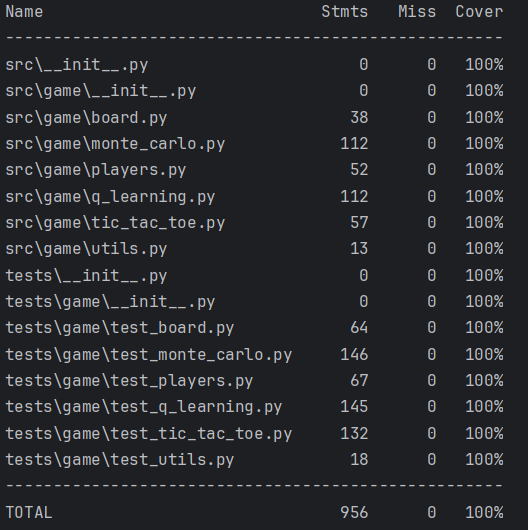
\includegraphics[width=0.5\textwidth]{./Figures/coverage.png}
	\caption{Reporte de cobertura.}
	\label{fig:coverage}
\end{figure}

Para mantener una buena calidad de código se ejecutaron análisis estáticos mediante la herramienta SonarLint y se resolvieron las malas prácticas y los problemas de seguridad encontrados.

\begin{figure}[htbp]
	\centering
	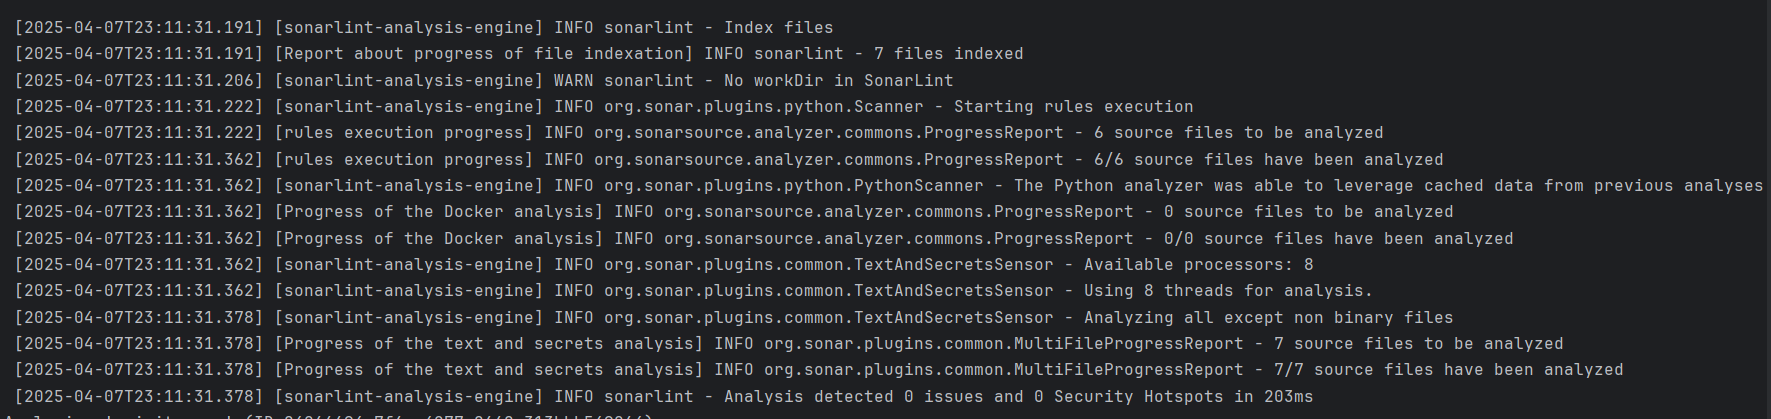
\includegraphics[width=\textwidth]{./Figures/sonar.png}
	\caption{Análisis estático de código.}
	\label{fig:coverage}
\end{figure}

